% OrthoHPI 2.0 manuscript.
%
% Build with `make` (needs tectonic: brew install tectonic).
% refs.bib is exported from Zotero -- do not edit it by hand, add the
% reference in Zotero instead. See the Makefile header.

\documentclass[11pt,a4paper]{article}

\usepackage[T1]{fontenc}
\usepackage[utf8]{inputenc}
\usepackage{lmodern}
\usepackage{microtype}

% 15 mm side margins make the text block 180 mm, the two-column width the
% figures are built at (scripts/figure_style.py), so they render at full size.
\usepackage[a4paper,left=1.5cm,right=1.5cm,top=2cm,bottom=2cm]{geometry}
\usepackage{graphicx}
\usepackage{booktabs}
\usepackage{longtable}
\usepackage{pdflscape}
\usepackage{array}
% Left-aligned, ragged paragraph column for the generated tables.
\newcolumntype{L}[1]{>{\raggedright\arraybackslash}p{#1}}
\usepackage{siunitx}
\usepackage{authblk}
\usepackage[hidelinks]{hyperref}
\usepackage[table]{xcolor}
% Every second row of the generated tables.
\definecolor{rowblue}{HTML}{E8F1FB}

% natbib + classic bibtex rather than biblatex + biber: tectonic runs bibtex
% internally, but has to shell out to biber, and its bundled biblatex (3.17)
% does not match the biber Homebrew ships (2.22). natbib is also what most
% journal classes expect, so this survives the move to a template.
\usepackage[numbers,sort&compress]{natbib}
\bibliographystyle{unsrtnat}

\graphicspath{{figures/}}

% Preprint styling: line numbers and 1.5 spacing make a draft easier to
% comment on. Drop both when a journal class takes over.
\usepackage{lineno}
\linenumbers
\usepackage{setspace}
\onehalfspacing
% Captions stay single-spaced and small, so that a full-page figure and its
% caption still fit on one page at 1.5 spacing.
\usepackage{caption}
\captionsetup{font={small,stretch=1.0}}

% A note to self that survives into the PDF but is obviously not prose.
\newcommand{\todo}[1]{\textcolor{red}{[TODO: #1]}}

\title{OrthoHPI 2.0: homology-derived host--parasite protein--protein
interactions at tissue and cell-type resolution}

% Author list and affiliations as given on the EMBL poster
% (scripts/build_poster.py on branch poster-embl).
\author[1]{Ida K.S. Meitil}
\author[2]{Yesid Cuesta Astroz}
\author[2]{Juan Esteban Vargas Gomez}
\author[1]{Alberto Santos}
\affil[1]{Department of Health Technology, Technical University of Denmark,
Kgs.\ Lyngby, Denmark}
\affil[2]{Escuela de Microbiolog\'ia, Universidad de Antioquia, Medell\'in,
Colombia}

\date{\today}

\begin{document}

\maketitle

\begin{abstract}
\todo{abstract}
\end{abstract}

\section{Introduction}
OrthoHPI 2.0 renews and extends the original OrthoHPI
resource~\cite{cuestaastroz2019analysis}, integrating current releases of the
underlying databases and predictors and broadening the set of parasites
covered. Host proteins are restricted to surface-exposed localisations
predicted by DeepLoc~\cite{dum2024deeploc}.

\todo{introduction}

\section{Methods}

% The stages below mirror docs/pipeline.md, which is the running description
% of what `python -m pipeline.main` actually does. Keep the two in step.

Figure~\ref{fig:workflow} gives an overview of the prediction workflow: the
host and parasite proteomes are filtered by tissue expression and predicted
subcellular localisation, and interactions are then transferred between the
remaining proteins through shared orthologous groups.

% paper/figures/workflow.png is exported from workflow.svg: `make figures`.
\begin{figure}[htbp]
  \centering
  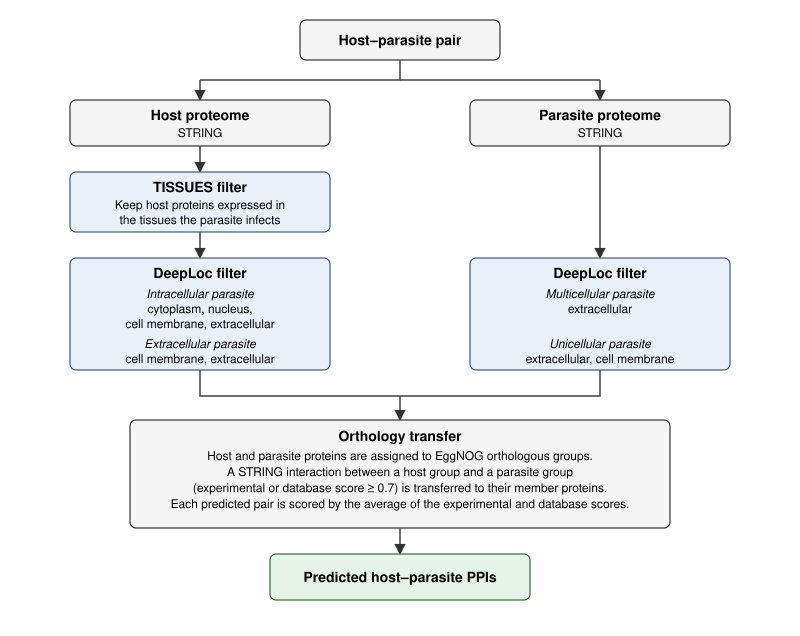
\includegraphics[width=\textwidth]{figures/workflow}
  \caption{Overview of the OrthoHPI 2.0 prediction workflow. For each
  host--parasite pair, the host proteome is restricted to proteins expressed in
  the tissues the parasite infects (TISSUES) and to localisations the parasite
  can reach (DeepLoc), and the parasite proteome to extracellular and, for
  unicellular parasites, cell-membrane proteins. STRING interactions between
  EggNOG orthologous groups are transferred to the remaining host and parasite
  proteins, each predicted pair scored by the mean of the experimental and
  database evidence scores.}
  \label{fig:workflow}
\end{figure}

\subsection{Data sources}
\todo{STRING v12.0, EggNOG 6, JensenLab TISSUES, Human Protein Atlas, Gene
Ontology. Canonical URLs and versions are in config.yml lines 1--32.}

\subsection{Proteomes and orthologous groups}
\todo{EggNOG Eukaryota (2759) groups; hosts human, rat, mouse, pig.}
The 45 parasite species, their hosts and the tissues they occupy are listed in
Table~\ref{tab:parasites}.

% paper/tables/parasites.tex is generated: `make tables` (see Makefile).
% Generated by scripts/build_parasite_table.py -- do not edit by hand.
\clearpage
\singlespacing\scriptsize
\setlength{\LTcapwidth}{\textwidth}
\rowcolors{2}{rowblue}{white}
\begin{longtable}{@{}L{3.95cm}cc L{2.6cm}L{8.6cm}@{}}
\caption{Parasites included in OrthoHPI 2.0, ordered by taxonomic group. U/M: unicellular or multicellular; I/E: intracellular or extracellular niche in the host; tissues are those the parasite occupies in the host during its lifecycle.}\label{tab:parasites}\\
\toprule
Species & U/M & I/E & Hosts & Tissues\\
\midrule
\endfirsthead
\multicolumn{5}{@{}l}{\textit{Table~\ref{tab:parasites} continued}}\\
\toprule
Species & U/M & I/E & Hosts & Tissues\\
\midrule
\endhead
\midrule
\multicolumn{5}{r@{}}{\textit{continued on next page}}\\
\endfoot
\bottomrule
\endlastfoot
\textit{Ancylostoma ceylanicum} & M & E & human & skin, lung, small intestine, intestine\\
\textit{Angiostrongylus cantonensis} & M & E & rat, mouse & lung, brain\\
\textit{Angiostrongylus costaricensis} & M & E & rat, mouse & mesenteric artery, intestine, blood\\
\textit{Brugia malayi} & M & E & human & lymph vessel, lymph node, blood\\
\textit{Brugia timori} & M & E & human & lymph vessel, lymph node, blood\\
\textit{Dracunculus medinensis} & M & E & human & small intestine, intestine, skin\\
\textit{Enterobius vermicularis} & M & E & human & colon, intestine, skin\\
\textit{Loa loa} & M & E & human & skin, blood, eye\\
\textit{Necator americanus} & M & E & human & skin, lung, small intestine, intestine\\
\textit{Nippostrongylus brasiliensis} & M & E & rat, mouse & skin, blood, lung, small intestine, intestine\\
\textit{Onchocerca volvulus} & M & E & human & skin, eye\\
\textit{Strongyloides stercoralis} & M & E & human & skin, lung, small intestine, intestine\\
\textit{Toxocara canis} & M & E & human & liver, heart, lung, brain, muscle, eye\\
\textit{Trichinella britovi} & M & I & human & intestine, muscle, brain, heart, lung\\
\textit{Trichinella nativa} & M & I & human & intestine, muscle, brain, heart, lung\\
\textit{Trichinella nelsoni} & M & I & human & intestine, muscle, brain, heart, lung\\
\textit{Trichinella pseudospiralis} & M & I & human, pig & intestine, muscle, brain, heart, lung\\
\textit{Trichinella spiralis} & M & I & human, pig & intestine, brain, heart, muscle, lung\\
\textit{Trichuris trichiura} & M & E & human & colon, intestine\\
\textit{Wuchereria bancrofti} & M & E & human & blood, lymph node, lymph vessel\\
\textit{Clonorchis sinensis} & M & E & human & liver, bile duct\\
\textit{Opisthorchis felineus} & M & E & human & liver, bile duct, small intestine, intestine\\
\textit{Opisthorchis viverrini} & M & E & human & liver, bile duct\\
\textit{Schistosoma haematobium} & M & E & human & skin, urinary bladder, rectum, intestine, liver, blood, lung\\
\textit{Schistosoma japonicum} & M & E & human & skin, liver, small intestine, intestine, lung, blood\\
\textit{Schistosoma mansoni} & M & E & human & skin, liver, intestine, spleen, lung, blood\\
\textit{Echinococcus granulosus} & M & E & human & liver, lung\\
\textit{Echinococcus multilocularis} & M & E & human & liver, lung\\
\textit{Hymenolepis diminuta} & M & E & human, rat, mouse & small intestine, intestine\\
\textit{Taenia asiatica} & M & E & human & small intestine, intestine\\
\textit{Cryptosporidium muris} & U & I & human, rat, mouse & stomach, intestine\\
\textit{Cryptosporidium parvum} & U & I & human & small intestine, intestine\\
\textit{Plasmodium falciparum} & U & I & human & skin, liver, blood, brain, spleen\\
\textit{Plasmodium knowlesi} & U & I & human & skin, liver, blood\\
\textit{Plasmodium vivax} & U & I & human & skin, liver, blood\\
\textit{Toxoplasma gondii} & U & I & human & blood, brain, eye, heart, muscle, placenta, lymph node\\
\textit{Leishmania braziliensis} & U & I & rat, mouse & skin, nose, mouth, macrophage, blood\\
\textit{Leishmania infantum} & U & I & human & liver, spleen, bone marrow, lymph node, skin, blood, macrophage\\
\textit{Leishmania major} & U & I & human & skin, blood, macrophage\\
\textit{Trypanosoma brucei} & U & E & human & skin, blood, brain, lymph node, spinal cord\\
\textit{Trypanosoma cruzi} & U & I & human & skin, heart, colon, intestine, muscle, blood, eye\\
\textit{Entamoeba histolytica} & U & E & human & colon, intestine, liver, brain, lung\\
\textit{Giardia lamblia} & U & E & human & small intestine, intestine\\
\textit{Trichomonas vaginalis} & U & E & human & vagina, urethra, uterine cervix, prostate, urinary tract\\
\textit{Trachipleistophora hominis} & U & I & human & muscle, eye\\
\textit{Vittaforma corneae} & U & I & human & eye\\
\end{longtable}


\subsection{Filtering the parasite proteome}
\todo{Secretome filter via DeepLoc.}

\subsection{Filtering the host proteome}
\todo{Tissue filter against parasite lifecycle tissues; DeepLoc filter to
surface-exposed localisations.}

\subsection{Homology transfer}
\todo{Transfer of STRING interactions through shared orthologous groups.}

Figure~\ref{fig:funnel} quantifies the filters of Figure~\ref{fig:workflow},
stage by stage and separately for each host--parasite pair. The DeepLoc filter
leaves an intracellular parasite roughly five times as many host proteins as an
extracellular one.

% paper/figures/funnel.pdf is generated: `make figures` (see Makefile).
\begin{figure}[p]
  \centering
  \includegraphics[width=\textwidth,height=0.83\textheight,keepaspectratio]{figures/funnel}
  \caption{Proteins surviving each stage of the pipeline, for every
  host--parasite pair. Bars are nested on a logarithmic axis, one row per pair,
  in blocks by host. The host side (left) runs from the STRING proteome through
  the TISSUES and DeepLoc filters to the proteins in a predicted interaction
  with that parasite; the parasite side (right) from the STRING proteome
  through the DeepLoc secretome filter and assignment to an EggNOG orthologous
  group to the proteins in a predicted interaction with that host. Both filters
  keep what Figure~\ref{fig:workflow} specifies. The orthologous-group stage is
  omitted on the host side, where every protein reaching it is already in a
  group. Rows are ordered by the parasite's niche in the host, then taxonomic
  group, then name; the strips left of each block give the niche (outer) and
  the taxonomic group (inner). The counts behind every row, and the number of
  predicted interactions of each pair, are in Supplementary Table~S1.}
  \label{fig:funnel}
\end{figure}

\subsection{Tissue and cell-type annotation}
\todo{TISSUES confidence scores and HPA single-cell expression.}

\subsection{Implementation and availability}
\todo{Streamlit application, repository URL, data snapshot.}

\section{Results}

\subsection{The predicted networks}
\todo{Size of the networks; what drives the spread between parasites.}
Figure~\ref{fig:networks} shows the size of each predicted network and where in
the host cell its interactions land.

% paper/figures/networks.pdf is generated: `make figures` (see Makefile).
\begin{figure}[p]
  \centering
  \includegraphics[width=\textwidth,height=0.83\textheight,keepaspectratio]{figures/networks}
  \caption{Predicted interactions of every host--parasite pair, one block per
  host, the blocks sharing an axis so that a bar is comparable across hosts.
  Each bar is split by where DeepLoc places the host protein: on the surface
  (extracellular or cell membrane), in the interior (cytoplasm or nucleus), or
  called for both. The interior fraction is what the parasite's niche opens to
  it, so it is substantial only for the intracellular parasites. The strips
  beside the names give the niche (outer) and the taxonomic group (inner).}
  \label{fig:networks}
\end{figure}

\subsection{Parasites of the same host reach overlapping host proteins}
\todo{Interpretation: similarity within genera and within niches.}
Figure~\ref{fig:similarity} compares the interactomes of the parasites of human
pair by pair, and Figure~\ref{fig:shared_families} the host families that the
most of them converge on.

% paper/figures/parasite_similarity.pdf is generated: `make figures`.
\begin{figure}[p]
  \centering
  \includegraphics[width=\textwidth,height=0.83\textheight,keepaspectratio]{figures/parasite_similarity}
  \caption{Jaccard similarity of the sets of human proteins reached by each
  pair of parasites predicted against human. Parasites are ordered by niche in
  the host, then taxonomic group, then name, so that the two niches read as
  blocks; the strips along both axes give the niche (outer) and the taxonomic
  group (inner), and the diagonal is left grey. Similarity is highest within a
  genus and falls away sharply between the niches, which draw on different host
  localisations.}
  \label{fig:similarity}
\end{figure}

% paper/figures/shared_families.pdf is generated: `make figures`.
\begin{figure}[p]
  \centering
  \includegraphics[width=\textwidth,height=0.83\textheight,keepaspectratio]{figures/shared_families}
  \caption{Host protein families of human reached by at least twelve
  parasites, as a dot matrix over the parasites predicted against human. A
  family is the orthologous group of the host protein, labelled by the gene
  symbols of its members, and is reached by a parasite when any parasite
  protein is predicted to interact with any member. The area of a dot is the
  number of parasite proteins reaching that family. The three columns on the
  right count the parasites reaching the family, the distinct parasite
  orthologous groups they do so through --- one group means a single conserved
  parasite protein transferred many times, rather than independent convergence
  --- and the split between helminths and protozoa. The strips above the matrix
  give the niche (outer) and the taxonomic group (inner).}
  \label{fig:shared_families}
\end{figure}

\subsection{Comparing the hosts of one parasite}
\todo{Interpretation: how much of a parasite's interactome is host specific.}
Figure~\ref{fig:multi_host} compares, for each parasite predicted against more
than one host, which interactions are shared and why the others are missing.

% paper/figures/multi_host.pdf is generated: `make figures`.
\begin{figure}[htbp]
  \centering
  \includegraphics[width=\textwidth]{figures/multi_host}
  \caption{Hosts compared for every parasite predicted against more than one.
  An interaction is compared between hosts as the pair of orthologous groups it
  was transferred from, so a link counts as shared when both hosts carry a
  protein of the host group interacting with the parasite's. \textbf{(A)} The
  links of each parasite, split by the hosts carrying them. \textbf{(B)} For
  each host, the links it lacks that another host of the same parasite carries,
  attributed to the first filter the host family fails there: the family is
  absent from the host proteome, no member is expressed in a tissue the
  parasite infects, no expressed member is in a location the parasite reaches,
  or the family is available and STRING transferred nothing.}
  \label{fig:multi_host}
\end{figure}

\subsection{From parasite protein to host cell type}
\todo{Interpretation of the \textit{Necator americanus} case study.}
Figure~\ref{fig:case_study} follows one pair from the parasite protein family
to the host cell types expressing its targets.

% paper/figures/case_study.pdf is generated: `make figures`.
\begin{figure}[p]
  \centering
  \includegraphics[width=\textwidth,height=0.83\textheight,keepaspectratio]{figures/case_study}
  \caption{\textit{Necator americanus} in \textit{Homo sapiens}.
  \textbf{(A)} Predicted interactions between parasite orthologous groups
  (rows, named by the commonest description of their members, with the number
  of parasite proteins in parentheses) and human proteins (columns), coloured
  by the confidence score of the prediction. Families reaching fewer than three
  host proteins are left out. \textbf{(B)} Expression of the same host
  proteins, sharing the columns of (A), across the cell types of the tissues
  the parasite infects, from the Human Protein Atlas. The eight cell types of
  each tissue expressing the most of these host proteins are kept, and the
  strip beside the names gives the tissue.}
  \label{fig:case_study}
\end{figure}

\section{Discussion}
\todo{discussion}

\section*{Supplementary material}
\textbf{Supplementary Table S1} (\texttt{funnel\_supplementary.csv}). One row
per host--parasite pair, in the order Figure~\ref{fig:funnel} draws them: the
host and parasite proteins surviving each stage of the pipeline, and the number
of predicted interactions of the pair. Supplied as a comma-separated file
rather than typeset, since the 56 rows are meant to be sorted and filtered.

\section*{Data and code availability}
\todo{Repository: \url{https://github.com/Multiomics-Analytics-Group/OrthoHPI2.0}}

\bibliography{refs}

\end{document}
